\documentclass[svgnames,11pt]{beamer}
\input{/home/tof/Documents/Cozy/latex-include/preambule_commun.tex}
\input{/home/tof/Documents/Cozy/latex-include/preambule_beamer.tex}
%\usepackage{pgfpages} \setbeameroption{show notes on second screen=left}
\author[]{Christophe Viroulaud}
\title{TP rotation image}
\date{\framebox{\textbf{Algo 03}}}
%\logo{}
\institute{Terminale - NSI}

\begin{document}
\begin{frame}
    \titlepage
\end{frame}
\begin{frame}
    \frametitle{}

    La rotation d'une image est une fonctionnalité proposée par n'importe quel logiciel de retouche tel \emph{Gimp}. L'opération n'est cependant pas triviale et peut demander une durée non négligeable.

\end{frame}
\begin{frame}
    \frametitle{}

    \begin{framed}\centering
        Construire un algorithme de rotation d'une image en appliquant le principe de \emph{diviser pour régner}.
    \end{framed}

\end{frame}
\section{Principe}
\begin{frame}
    \frametitle{Principe}

    \emph{Diviser pour régner} se décompose en trois parties:
    \begin{itemize}
        \item \emph{diviser:} Le problème est partagé en plusieurs petits problèmes identiques.
        \item \emph{traitement:} Chaque petit problème est résolu.
        \item \emph{recombinaison:} Les petits problèmes résolus sont assemblés pour remonter au problème principal.
    \end{itemize}

\end{frame}
\begin{frame}
    \frametitle{}

    \begin{activite}
        \textbf{Réflexion commune:} Considérons une image aux dimensions connues. Quelles étapes pourrions-nous imaginer pour répondre à notre problématique?
    \end{activite}

\end{frame}
\begin{frame}
    \frametitle{Avant de regarder la correction}
    \begin{center}
        \centering
        \includegraphics[width=3cm]{/home/tof/Documents/Cozy/latex-include/stop.png}
    \end{center}
    {\Large
    \begin{itemize}
        \item Prendre le temps de réfléchir,
        \item Analyser les messages d'erreur,
        \item Demander au professeur.
    \end{itemize}
    }
\end{frame}
\begin{frame}
    \frametitle{Correction}

    \begin{center}
        \centering
        
\includegraphics[width=2cm]{ressources/carre0.png}
        \captionof{figure}{1 pixel: rien à faire}
        \label{IMG}
    \end{center}

\end{frame}
\begin{frame}
    \frametitle{Correction}

    \begin{center}
        \begin{tabular}{ccc}
            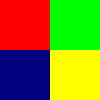
\includegraphics[width=3cm]{ressources/carre1.png}
             & $$\rightarrow$$
             &
            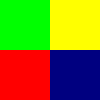
\includegraphics[width=3cm]{ressources/carre1-rot.png}
            \\
        \end{tabular}
        \captionof{figure}{Rotation}
    \end{center}
    \note{pixel(l=0, c=0) $\rightarrow$ (l=1, c=0)}
\end{frame}
\begin{frame}
    \frametitle{Correction}

    \begin{center}
        \begin{tabular}{ccccc}
            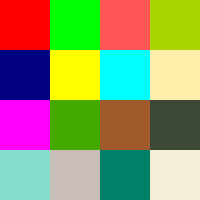
\includegraphics[width=2.5cm]{ressources/carre2.png}
             & $$\rightarrow$$
             &
            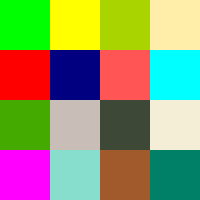
\includegraphics[width=2.5cm]{ressources/carre2-int.png}
             & $$\rightarrow$$
             &
            
\includegraphics[width=2.5cm]{ressources/carre2-rot.png}
            \\
        \end{tabular}
        \captionof{figure}{Récursivité: on divise la taille des problèmes par 2.}
    \end{center}

\end{frame}
\begin{frame}
    \frametitle{}

    \begin{itemize}
        \item Si la taille \texttt{\textbf{t}} est égal à 1, ne rien faire.
        \item Sinon: \textbf{découper en sous problèmes}
              \begin{itemize}
                  \item diviser la taille \textbf{\texttt{t}} en 2,
                  \item effectuer récursivement la rotation des \textbf{quatre parties} de la portion carrée comprise entre (x,y) et (x+t, y+t)
              \end{itemize}
        \item \textbf{résoudre les petits problèmes:} Effectuer la rotation des pixels.
    \end{itemize}

\end{frame}
\section{Algorithme de rotation}
\subsection{Chargement de l'image}
\begin{frame}[fragile]
    \frametitle{Chargement de l'image}

    \emph{PIL (Python Image Library) -anciennement pillow-} est une bibliothèque de traitement d'image.
    \begin{center}
        \begin{lstlisting}[language=Python , basicstyle=\ttfamily\small, xleftmargin=2em, xrightmargin=2em]
from PIL import Image

im = Image.open("image.png")
im.show()
\end{lstlisting}
        \captionof{code}{Charger une image}
        \label{CODE}
    \end{center}

\end{frame}
\begin{frame}[fragile]
    \frametitle{}

    \begin{center}
        \begin{lstlisting}[language=Python , basicstyle=\ttfamily\small, xleftmargin=2em, xrightmargin=2em]
largeur, hauteur = im.size
px = im.load()
\end{lstlisting}
        \captionof{code}{Récupérer des informations}
        \label{CODE}
    \end{center}
    \begin{aretenir}[Information]
        La variable \textbf{\texttt{px}} contient une matrice représentative des pixels de l'image. La couleur du pixel de coordonnées \textbf{\texttt{(x,y)}} est donnée par l'instruction \texttt{\textbf{px[x,y]}}. Il est également possible d'affecter une nouvelle couleur \textbf{\texttt{c}} à un pixel: \texttt{\textbf{px[x,y] = c}}.
    \end{aretenir}
\end{frame}
\begin{frame}
    \frametitle{}

    \begin{activite}
        \begin{enumerate}
            \item Récupérer une image carrée sur \url{https://www.freepng.fr/}.
            \item Charger et afficher cette image.
        \end{enumerate}
    \end{activite}

\end{frame}
\subsection{Résoudre un petit problème}
\begin{frame}
    \frametitle{Résoudre un petit problème}
    \begin{center}
        \begin{tabular}{cccc}
            {\Large $t=1$}
             &
            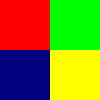
\includegraphics[width=2cm]{ressources/carre1.png}
             & $$\rightarrow$$
             &
            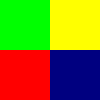
\includegraphics[width=2cm]{ressources/carre1-rot.png}
            \\
        \end{tabular}
    \end{center}
    \begin{center}
        \begin{tabular}{cccc}
            {\Large $t=2$}
             &
            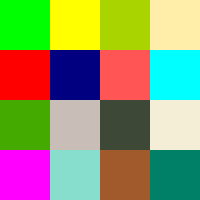
\includegraphics[width=2cm]{ressources/carre2-int.png}
             & $$\rightarrow$$
             &
            
\includegraphics[width=2cm]{ressources/carre2-rot.png}
            \\
        \end{tabular}
    \end{center}
    \begin{activite}
        Écrire la fonction \textbf{\texttt{tourner(px: object, x: int, y: int, t: int) $\rightarrow$ None}} qui effectue une rotation anti-horaire pour les pixels compris dans l'intervalle de colonnes $[x; x+t]$ et l'intervalle de lignes $[y; y+t]$.
    \end{activite}

\end{frame}
\begin{frame}
    \frametitle{Avant de regarder la correction}
    \begin{center}
        \centering
        \includegraphics[width=3cm]{/home/tof/Documents/Cozy/latex-include/stop.png}
    \end{center}
    {\Large
    \begin{itemize}
        \item Prendre le temps de réfléchir,
        \item Analyser les messages d'erreur,
        \item Demander au professeur.
    \end{itemize}
    }
\end{frame}
\begin{frame}[fragile]
    \frametitle{Correction}

    \begin{center}
        \begin{lstlisting}[language=Python , basicstyle=\ttfamily\small, xleftmargin=0em, xrightmargin=0em]
def tourner(px: object, x: int, y: int, t: int) -> None:
    for l in range(y, y+t):
        for c in range(x, x+t):
            px[l, c+t], px[l+t, c+t], \
            px[l+t, c], px[l, c] =\
                px[l, c], px[l, c+t], \
                px[l+t, c+t], px[l+t, c]
\end{lstlisting}
        \captionof{code}{Chaque \emph{bloc} tourne d'un cran dans le sens anti-horaire}
        \label{CODE}
    \end{center}

\end{frame}
\subsection{Diviser}
\begin{frame}
    \frametitle{Diviser}
    Partant d'une taille d'image \textbf{\texttt{t}} il faut diviser le problème en quatre problèmes plus petits.
    \begin{center}
        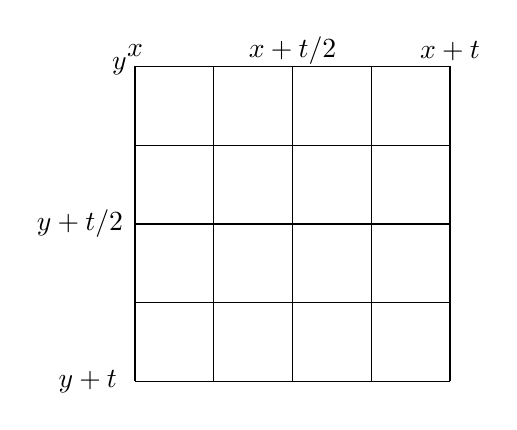
\begin{tikzpicture}
            \draw (0,0) grid (4,4);
            \node at (0,4.2) {$x$};
            \node at (2,4.2) {$x+t/2$};
            \node at (4,4.2) {$x+t$};
            \node at (-0.2,4) {$y$};
            \node at (-0.7,2) {$y+t/2$};
            \node at (-0.6,0) {$y+t$};

        \end{tikzpicture}
    \end{center}

\end{frame}
\begin{frame}
    \frametitle{Diviser}
    \begin{center}
        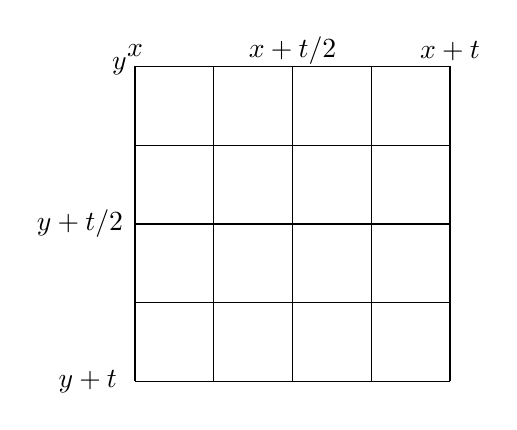
\begin{tikzpicture}
            \draw (0,0) grid (4,4);
            \node at (0,4.2) {$x$};
            \node at (2,4.2) {$x+t/2$};
            \node at (4,4.2) {$x+t$};
            \node at (-0.2,4) {$y$};
            \node at (-0.7,2) {$y+t/2$};
            \node at (-0.6,0) {$y+t$};

        \end{tikzpicture}
    \end{center}
    \begin{activite}
        Écrire la fonction récursive \textbf{\texttt{rotation(px: object, x: int, y: int, t: int) $\rightarrow$ None}} qui divise récursivement le problème en quatre, puis effectue la rotation à l'aide de la fonction \textbf{\texttt{tourner}}.
    \end{activite}
\end{frame}
\begin{frame}
    \frametitle{Avant de regarder la correction}
    \begin{center}
        \centering
        \includegraphics[width=3cm]{/home/tof/Documents/Cozy/latex-include/stop.png}
    \end{center}
    {\Large
    \begin{itemize}
        \item Prendre le temps de réfléchir,
        \item Analyser les messages d'erreur,
        \item Demander au professeur.
    \end{itemize}
    }
\end{frame}
\begin{frame}[fragile]
    \frametitle{Correction}

    \begin{center}
        \begin{lstlisting}[language=Python , basicstyle=\ttfamily\small, xleftmargin=2em, xrightmargin=2em]
def rotation(px: object, x: int, y: int, t: int) -> None:
    if t > 1:
        t //= 2
        rotation(px, x, y, t)
        rotation(px, x+t, y, t)
        rotation(px, x, y+t, t)
        rotation(px, x+t, y+t, t)

        tourner(px, x, y, t) 
\end{lstlisting}
        \captionof{code}{Le cas limite est atteint quand on a 1 seul pixel.}
        \label{CODE}
    \end{center}
    \begin{center}
        \begin{lstlisting}[language=Python , basicstyle=\ttfamily\small, xleftmargin=2em, xrightmargin=2em]
rotation(px, 0, 0, largeur)
\end{lstlisting}
        \captionof{code}{Appel principal}
        \label{CODE}
    \end{center}
\end{frame}
\section{Créer une bibliothèque}
\begin{frame}
    \frametitle{Créer une bibliothèque}

    Pour un utilisateur, le passage des différents paramètres (\textbf{\texttt{px}}, \textbf{\texttt{x}}, \textbf{\texttt{y}}, \textbf{\texttt{t}}) peut paraître fastidieux. Typiquement il ne devrait avoir à fournir qu'une information: le chemin du fichier image.

\end{frame}
\begin{frame}
    \frametitle{}

    \begin{activite}
        \begin{enumerate}
            \item Créer une classe \textbf{\texttt{Image\_perso}} et son constructeur qui admet un paramètre: le chemin de l'image. Ce constructeur construira alors un objet \textbf{\texttt{Image}} de la bibliothèque \textbf{\texttt{PIL}}.
            \item Écrire la méthode \textbf{\texttt{montrer}}, sans paramètre, qui affiche l'image.
            \item Écrire la méthode \textbf{\texttt{fait\_tourner}} sans paramètre, qui effectue une raotation anti-horaire de l'image. Il faudra adapter les fonctions construites précédemment pour en faire des méthodes internes à la classe.
            \item \textbf{Pour les plus avancés:} Adapter la méthode \textbf{\texttt{fait\_tourner}} qui acceptera un paramètre de type booléen. Si l'argument passé est \textbf{\texttt{True}} la rotation sera dans le sens horaire.
        \end{enumerate}
    \end{activite}

\end{frame}
\begin{frame}
    \frametitle{Avant de regarder la correction}
    \begin{center}
        \centering
        \includegraphics[width=3cm]{/home/tof/Documents/Cozy/latex-include/stop.png}
    \end{center}
    {\Large
    \begin{itemize}
        \item Prendre le temps de réfléchir,
        \item Analyser les messages d'erreur,
        \item Demander au professeur.
    \end{itemize}
    }
\end{frame}
\begin{frame}[fragile]
    \frametitle{Correction}

    \begin{center}
        \begin{lstlisting}[language=Python , basicstyle=\ttfamily\small, xleftmargin=2em, xrightmargin=2em]
class Image_lib:

    def __init__(self, fichier: str) -> None:
        self.image = Image.open(fichier)
        self.largeur, self.hauteur = self.image.size
        self.px = self.image.load()
\end{lstlisting}
        \captionof{code}{Constructeur}
        \label{CODE}
    \end{center}

\end{frame}
\begin{frame}[fragile]
    \frametitle{}

    \begin{center}
        \begin{lstlisting}[language=Python , basicstyle=\ttfamily\small, xleftmargin=2em, xrightmargin=2em]
def montrer(self):
    """
    affiche l'image
    """
    self.image.show()
\end{lstlisting}
        \captionof{code}{Afficher l'image}
        \label{CODE}
    \end{center}

\end{frame}
\begin{frame}[fragile]
    \frametitle{}

    \begin{center}
        \begin{lstlisting}[language=Python , basicstyle=\ttfamily\small, xleftmargin=2em, xrightmargin=2em]
def fait_tourner(self) -> None:
    """
    tourne l'image de 90° dans le sens anti-horaire sinon
    """
    self.rotation(0, 0, self.largeur)
\end{lstlisting}
        \captionof{code}{Il faut adapter la fonction \textbf{\texttt{rotation}.}}
        \label{CODE}
    \end{center}
    \begin{aretenir}[Remarque]
        Le paramètre \textbf{\texttt{px}} n'est plus nécessaire dans la méthode \textbf{\texttt{rotation}}. En effet, il est accessible depuis l'attribut crée dans le constructeur.
    \end{aretenir}
\end{frame}
\begin{frame}[fragile]
    \frametitle{}

    \begin{center}
        \begin{lstlisting}[language=Python , basicstyle=\ttfamily\small, xleftmargin=2em, xrightmargin=2em]
def rotation(self, x: int, y: int, t: int, horaire: bool) -> None:
    if t > 1:
        t //= 2
        self.rotation(x, y, t, horaire)
        self.rotation(x+t, y, t, horaire)
        self.rotation(x, y+t, t, horaire)
        self.rotation(x+t, y+t, t, horaire)

        self.tourner(x, y, t)
\end{lstlisting}
    \end{center}

\end{frame}
\begin{frame}[fragile]
    \frametitle{}

    \begin{center}
        \begin{lstlisting}[language=Python , basicstyle=\ttfamily\small, xleftmargin=.5em, xrightmargin=.5em]
def tourner(self, x: int, y: int, t: int) -> None:
    for l in range(y, y+t):
        for c in range(x, x+t):
            self.px[l, c+t], self.px[l+t, c+t], \
            self.px[l+t, c], self.px[l, c] = \
                self.px[l, c], self.px[l, c + t], \
                self.px[l+t, c+t], self.px[l+t, c]
\end{lstlisting}
    \end{center}

\end{frame}
\begin{frame}[fragile]
    \frametitle{}

    \begin{center}
        \begin{lstlisting}[language=Python , basicstyle=\ttfamily\small, xleftmargin=2em, xrightmargin=2em]
def fait_tourner(self, horaire: bool = True) -> None:
    """
    tourne l'image de 90°

    Paramètres
    -------
    horaire: booléen; défaut: True
        tourne de 90° dans le sens horaire si True,
        dans le sens anti-horaire sinon
    """
    self.rotation(0, 0, self.largeur, horaire)
\end{lstlisting}
        \captionof{code}{Avec choix de la rotation}
        \label{CODE}
    \end{center}

\end{frame}
\begin{frame}[fragile]
    \frametitle{}
    \begin{center}
        \begin{lstlisting}[language=Python , basicstyle=\ttfamily\small, xleftmargin=2em, xrightmargin=2em]
def rotation(self, x: int, y: int, t: int, horaire: bool) -> None:
    if t > 1:
        t //= 2
        self.rotation(x, y, t, horaire)
        self.rotation(x+t, y, t, horaire)
        self.rotation(x, y+t, t, horaire)
        self.rotation(x+t, y+t, t, horaire)

        if horaire:
            self.tourner_horaire(x, y, t)
        else:
            self.tourner_antihoraire(x, y, t)
\end{lstlisting}
        \captionof{code}{adaptation de \textbf{\texttt{rotation}}}
        \label{CODE}
    \end{center}


\end{frame}
\begin{frame}[fragile]
    \frametitle{}

    \begin{center}
        \begin{lstlisting}[language=Python , basicstyle=\ttfamily\small, xleftmargin=0.1em, xrightmargin=-0.4em]
def tourner_antihoraire(self, x: int, y: int, t: int) -> None:
    for l in range(y, y+t):
        for c in range(x, x+t):
            self.px[l, c+t], self.px[l+t, c+t], \
            self.px[l+t, c], self.px[l, c] = \
                self.px[l, c], self.px[l, c + t], \
                self.px[l+t, c+t], self.px[l+t, c]

def tourner_horaire(self, x: int, y: int, t: int) -> None:
    for l in range(y, y+t):
        for c in range(x, x+t):
            self.px[l, c+t], self.px[l+t, c+t], \
                self.px[l+t, c], self.px[l, c] = \
                self.px[l+t, c+t], self.px[l+t, c], \
                    self.px[l, c], self.px[l, c+t]
\end{lstlisting}
        \captionof{code}{Tourner}
        \label{CODE}
    \end{center}

\end{frame}
\end{document}